\documentclass[review]{elsarticle}
 \usepackage{fullpage}
 \usepackage{amsfonts} 
 \usepackage{amsmath}
 \usepackage{amsthm}
% \usepackage{amsrefs}
% \def\bibsection{\section*{References}}
 \usepackage{pifont}
 \usepackage{natbib}
 \usepackage{geometry}
 \usepackage{graphicx}
 \usepackage{hyperref}
 
%ming's package for numerical section 
\RequirePackage{lineno}
\usepackage{subfig}
\usepackage{amssymb}
\usepackage{multirow}
\usepackage{subfig}
\usepackage{setspace}
\usepackage{url}
\usepackage{color}

%environment
\newtheorem{thm}{Theorem}
\newtheorem{lem}[thm]{Lemma}
\newtheorem{cor}{Corollary}
\newdefinition{rmk}{Remark}
\newtheorem*{defi*}{Definition}
%\newproof{proof}{Proof}
\begin{document}

\begin{frontmatter}
\title{Ranking Distance Correlation}
%\author[jhuams]{CS, JV, CEP}

\end{frontmatter}

\section{Set-up}
Let $X \sim U(0,1)^{d} \in \mathbb{R}^{d}$, where $U$ is the uniform distribution, $d$ is the dimension size. 

Let $Y=f(A \times X) + \epsilon \in \mathbb{R}$, where $f: \mathbb{R} \rightarrow \mathbb{R}$ is a function of $X$, $A$ is a $1 \times d$ transformation, and $\epsilon$ is random noise. So $Y$ is a one-dimensional variable that is related to $X$.

For the choice of $f()$, we use linear, quadratic, cubic, sine period $1/2$, sine period $1/8$, $X^{0.25}$, circle, step function, exponential, and log function. Please see the code for detail. 

For the choice of $A$, we use $A(i)=1/i, \forall i=1,\ldots,d$, so that the entries of $A$ decays as the dimension increases. Note that we may also use a random decay rather than the fixed decay, and the numerical phenomenon is similar.

\section{Independence tests}
Given two sample data $\mathcal{X}$ and $\mathcal{Y}$ of size $d \times n$ and size $1 \times n$ ($n$ is the sample size), the null hypothesis is that they are not independent. The alternative hypothesis is they are independent.

Fix $f$ and $A$. To test whether our Ranking Distance Correlation improves over distance correlation, the experiment is done as follows: we first obtain $\mathcal{X}$ and $\mathcal{Y}$ by generating $(X,Y)$ for $n=100$ pairs, and calculate the distance correlation and Ranking Distance Correlation between them. Repeat it for $1000$ Monte-Carlo replicates, we obtain the empirical distribution of DC and RDC for that type of $f$ and $A$, which are the test statistics under the null.

Now repeat the same procedure, but $\mathcal{X}$ and $\mathcal{Y}$ are generated from $(Z,Y)$ for $n=100$ pairs. $Z \sim U(0,1)^{d} \in \mathbb{R}^{d}$ but is independent from $X$, so $Z$ is also independent from $Y$. After $1000$ Monte-Carlo replicates, we obtain the empirical distribution of DC and RDC under the alternative.

Given DC and RDC under the null and the alternative, we calculate the testing power at type $1$ error level $0.95$. To assess the effect for high-dimensional data, we do the experiment for $d=1,10,20,\ldots,1000$ at $n=100$. 

For the first subsection, we present the testing powers with $\epsilon=0$; but the performance is similar for small error as well. For the second subsection, we present the testing powers with increasing noise level (which is generated by Gaussian) at fixed $d=500$; the interpretation is similar for other dimensions as well. 

It is clear that RDC performs very similarly as DC for low-dimensional data; but for high-dimensional data we observe a clear advantage of RDC in testing independence. Such advantage is also robust against noise.

\section{Powers with respect to Dimension}

\begin{figure}[htbp]
\subfloat[]{
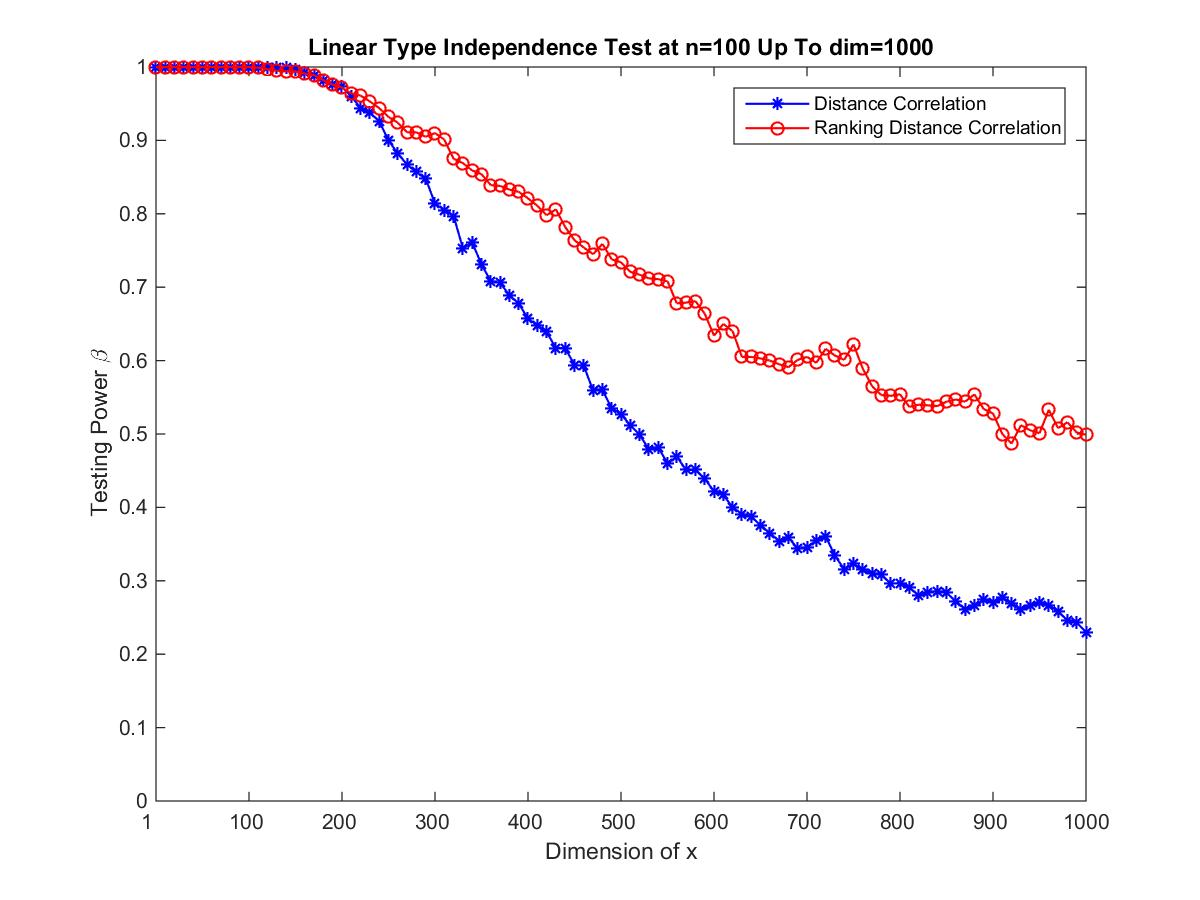
\includegraphics[width=0.5\textwidth]{data/fig1/TibsSimuInd2DimType1N100}
}
\hfil
\subfloat[]{
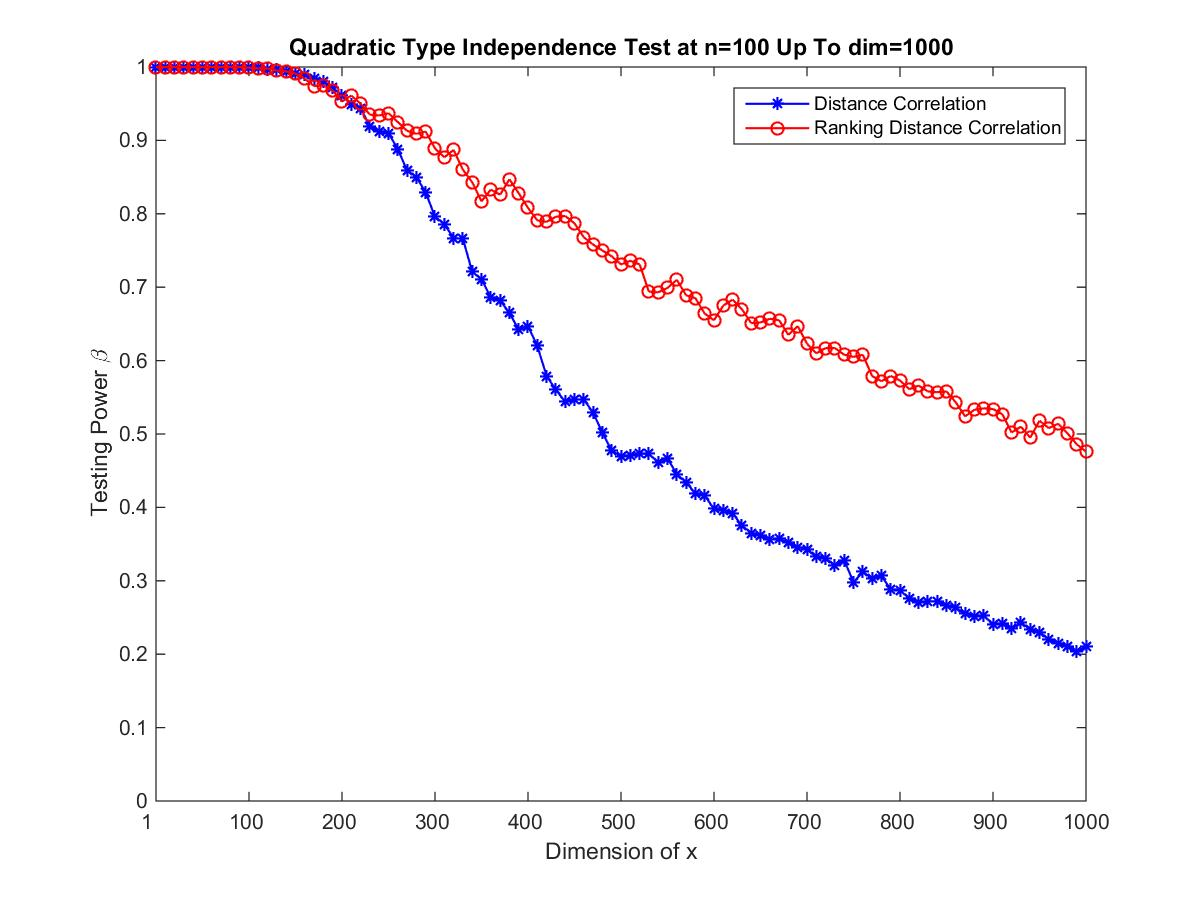
\includegraphics[width=0.5\textwidth]{data/fig1/TibsSimuInd2DimType2N100}
}
\hfil
\subfloat[]{
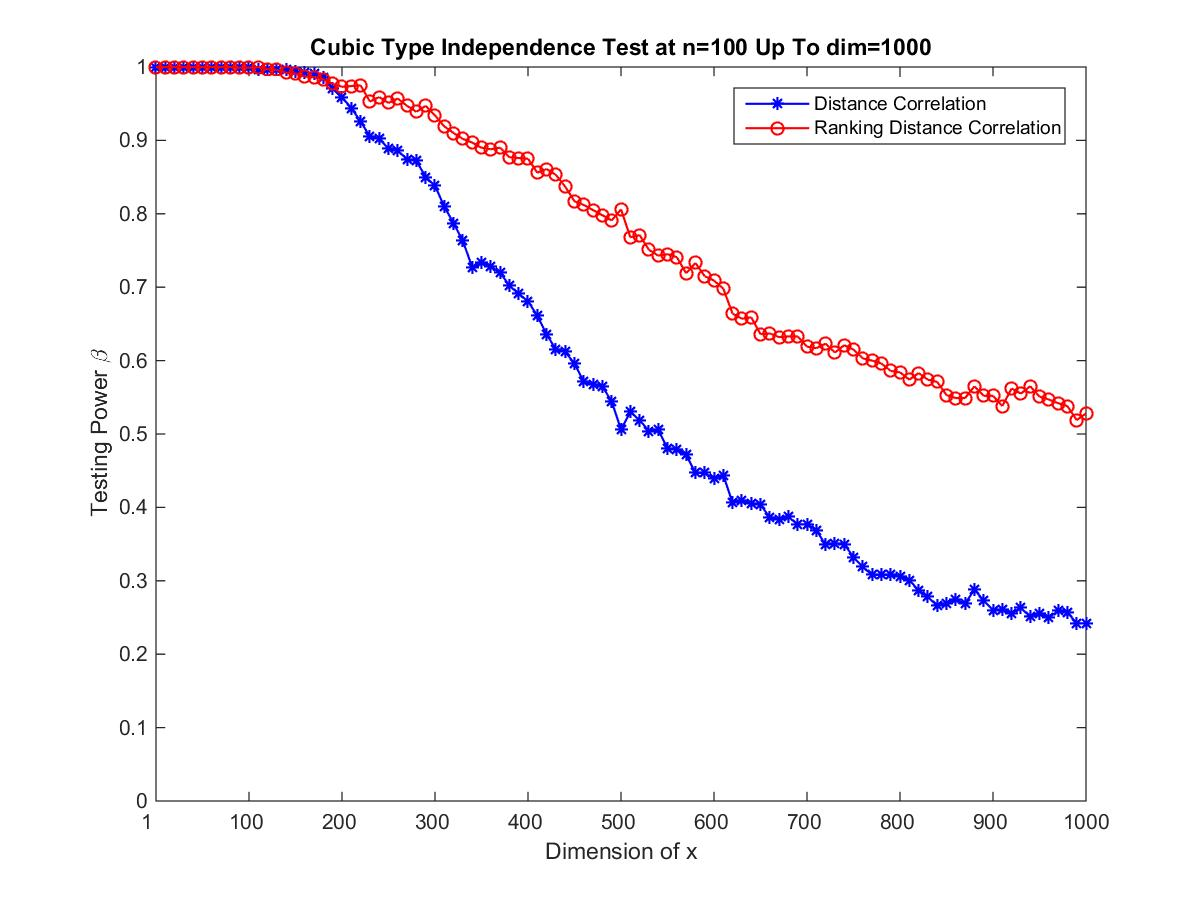
\includegraphics[width=0.5\textwidth]{data/fig1/TibsSimuInd2DimType3N100}
}
\hfil
\subfloat[]{
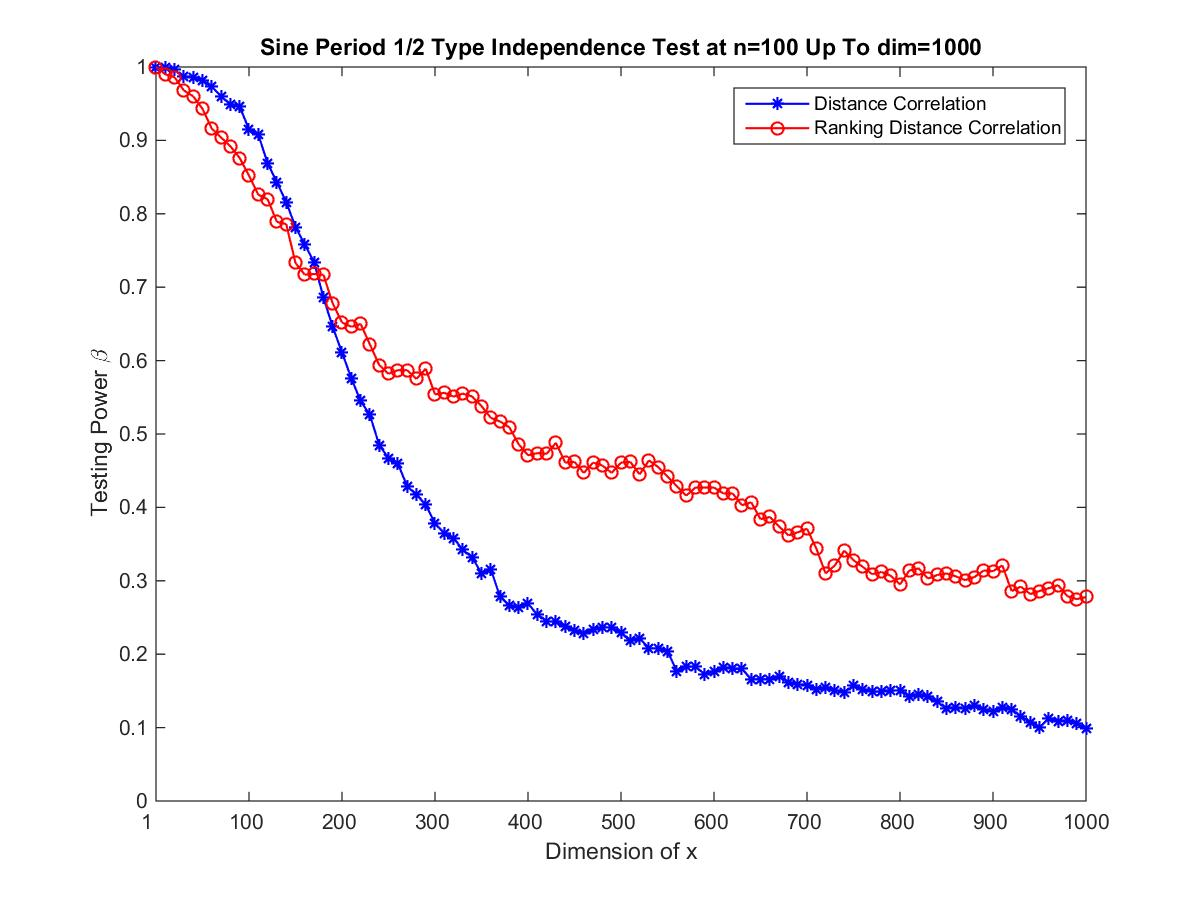
\includegraphics[width=0.5\textwidth]{data/fig1/TibsSimuInd2DimType4N100}
}
\hfil
\subfloat[]{
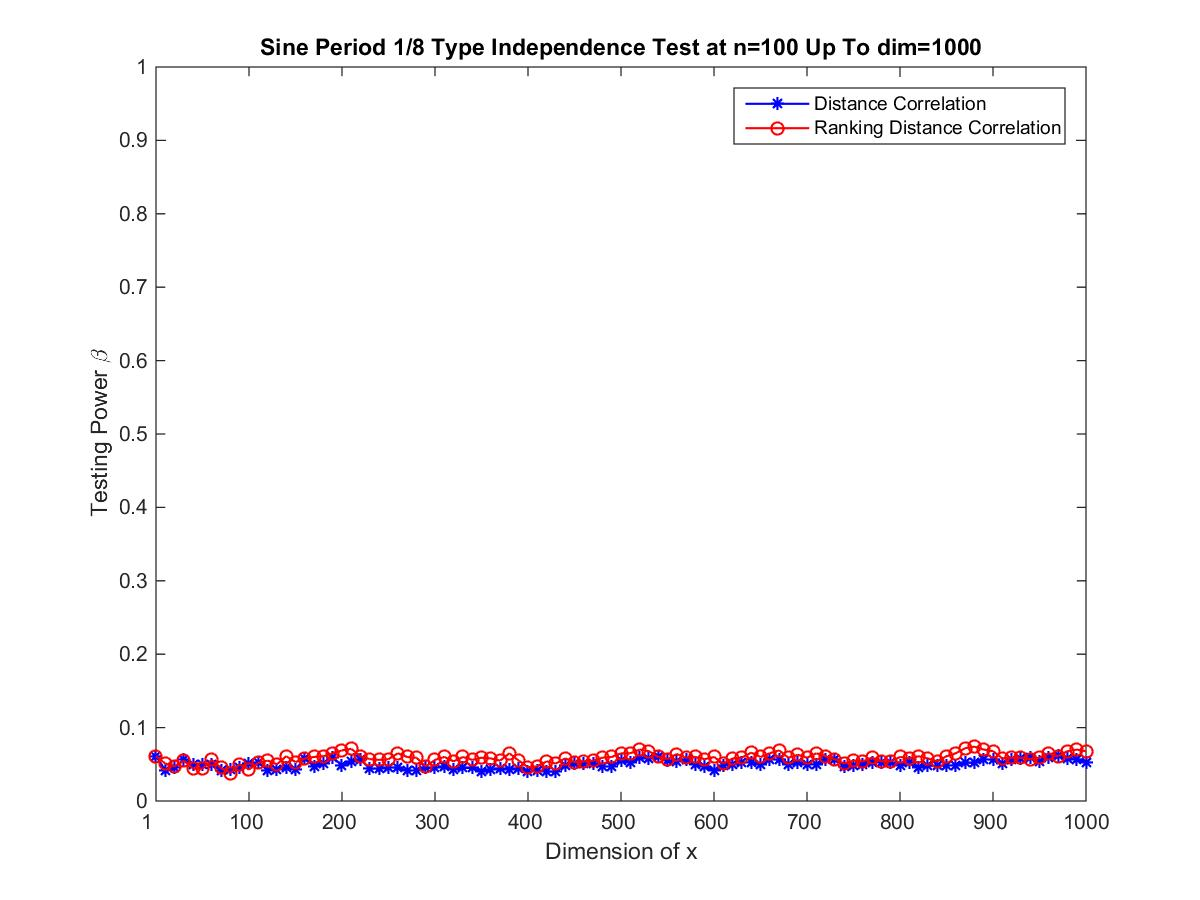
\includegraphics[width=0.5\textwidth]{data/fig1/TibsSimuInd2DimType5N100}
}
\hfil
\subfloat[]{
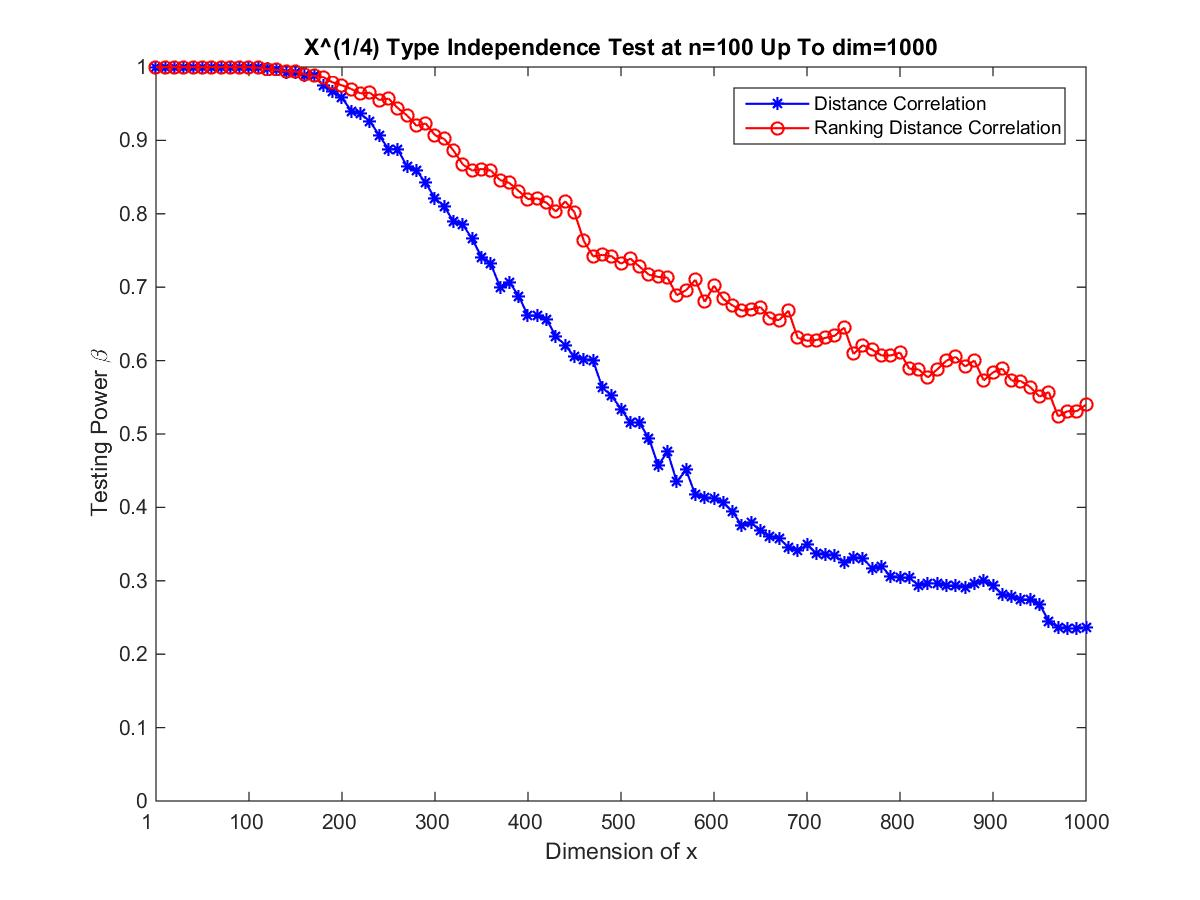
\includegraphics[width=0.5\textwidth]{data/fig1/TibsSimuInd2DimType6N100}
}
\caption{Testing Powers w.r.t. Increasing Dimension}
\label{}
\end{figure}

\begin{figure}[htbp]
\subfloat[]{
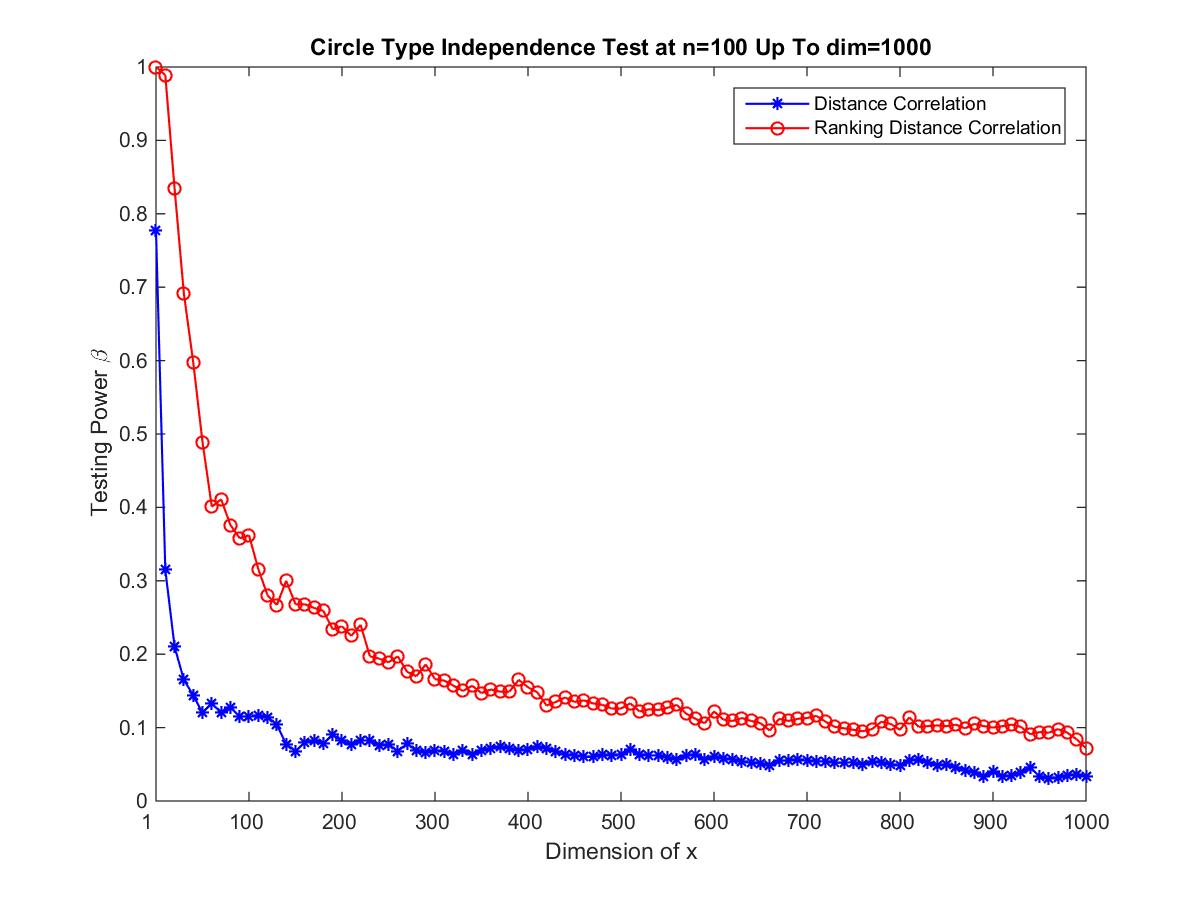
\includegraphics[width=0.5\textwidth]{data/fig1/TibsSimuInd2DimType7N100}
}
\hfil
\subfloat[]{
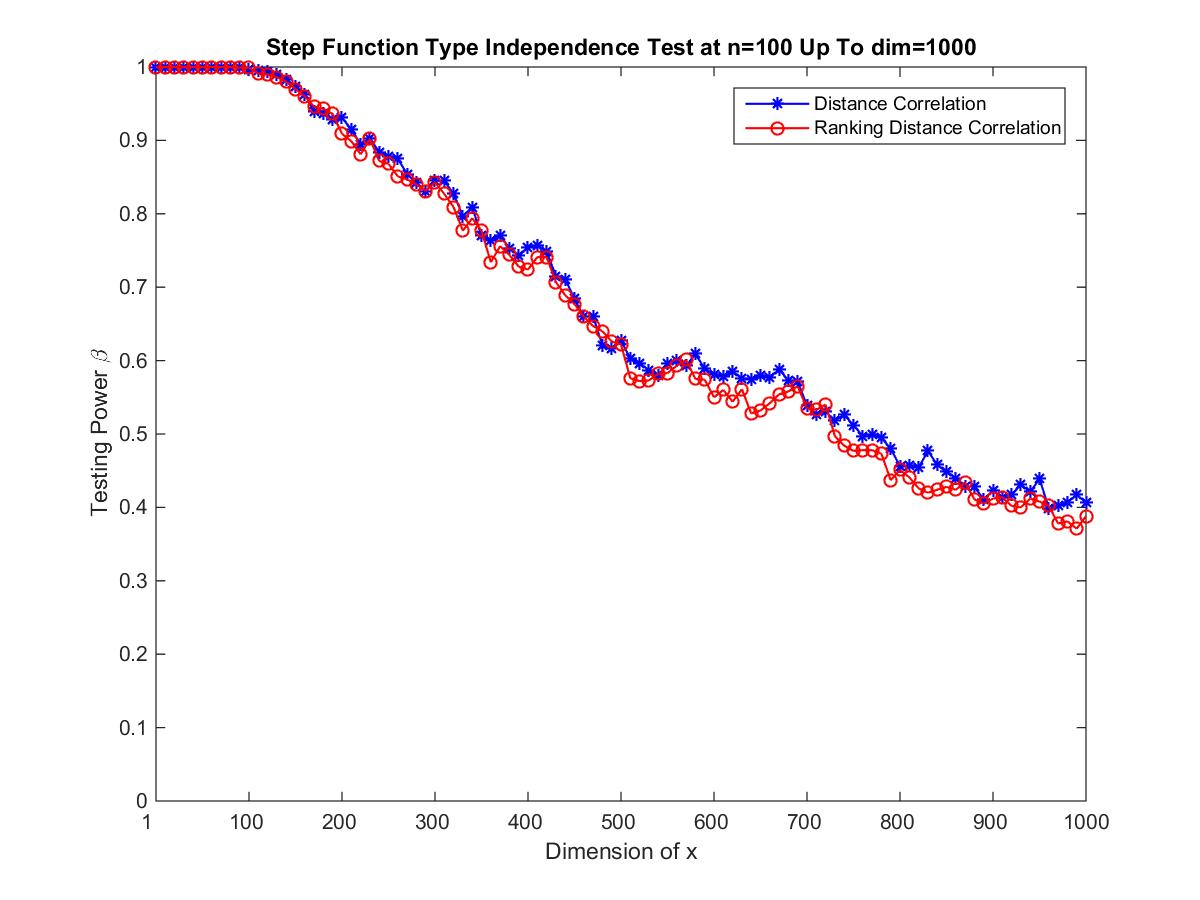
\includegraphics[width=0.5\textwidth]{data/fig1/TibsSimuInd2DimType8N100}
}
\hfil
\subfloat[]{
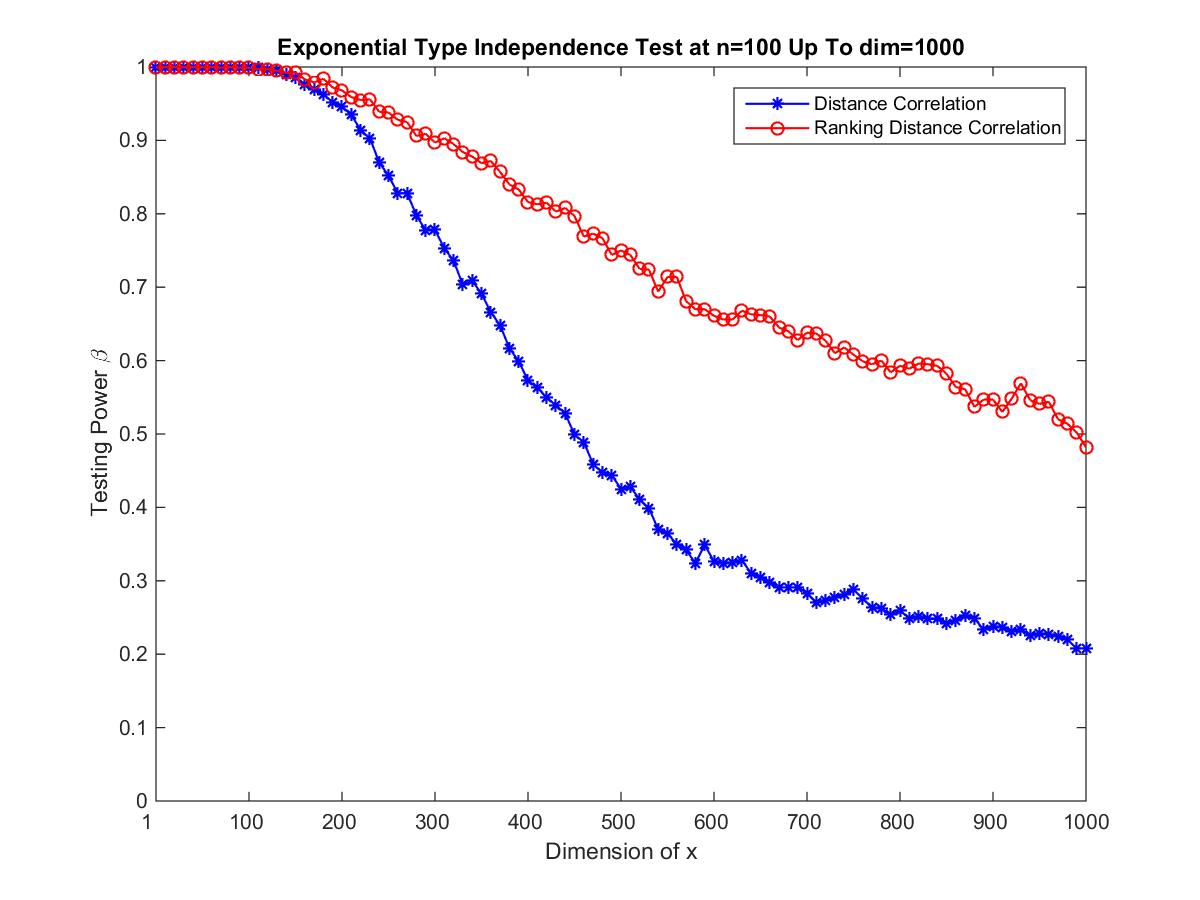
\includegraphics[width=0.5\textwidth]{data/fig1/TibsSimuInd2DimType9N100}
}
\hfil
\subfloat[]{
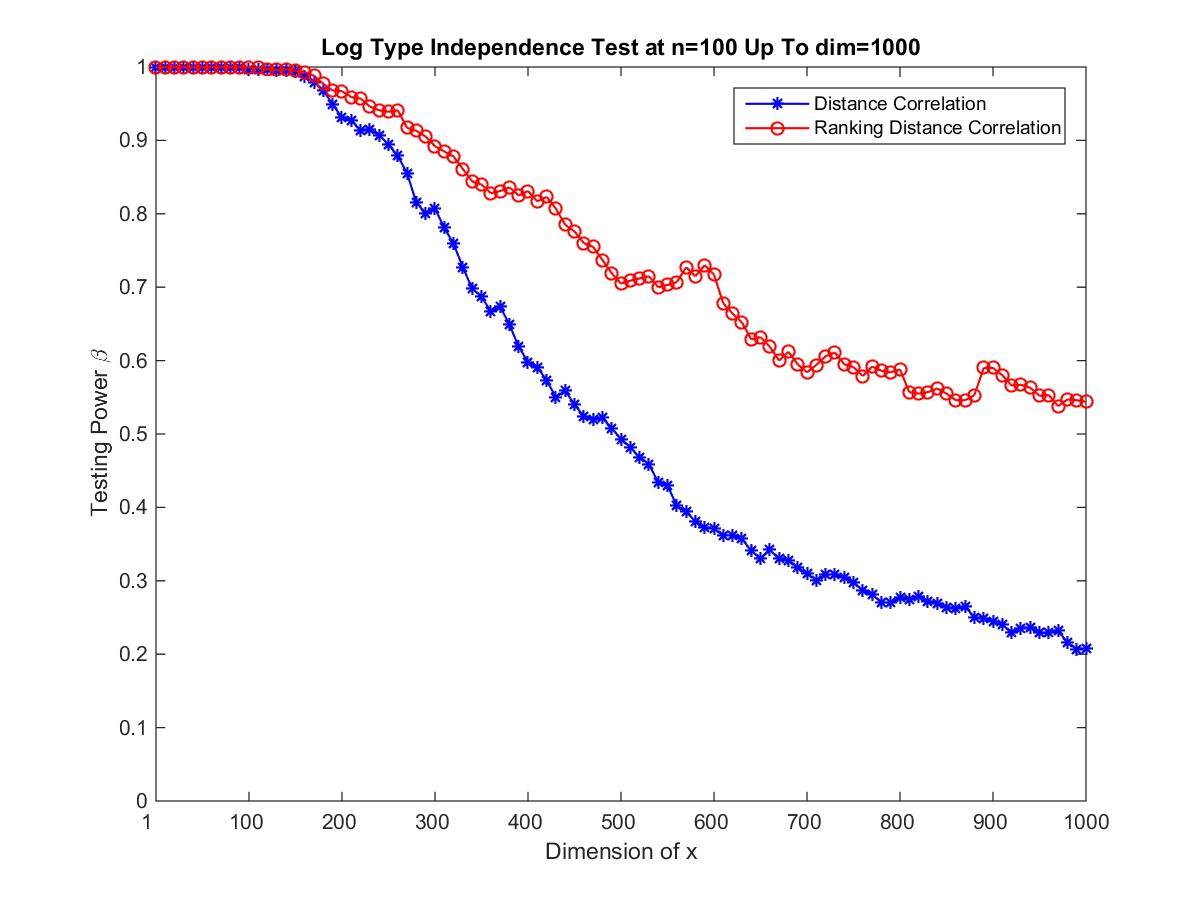
\includegraphics[width=0.5\textwidth]{data/fig1/TibsSimuInd2DimType10N100}
}
\caption{Testing Powers w.r.t. Increasing Dimension}
\label{}
\end{figure}

\section{Powers with respect to Noise}

\begin{figure}[htbp]
\subfloat[]{
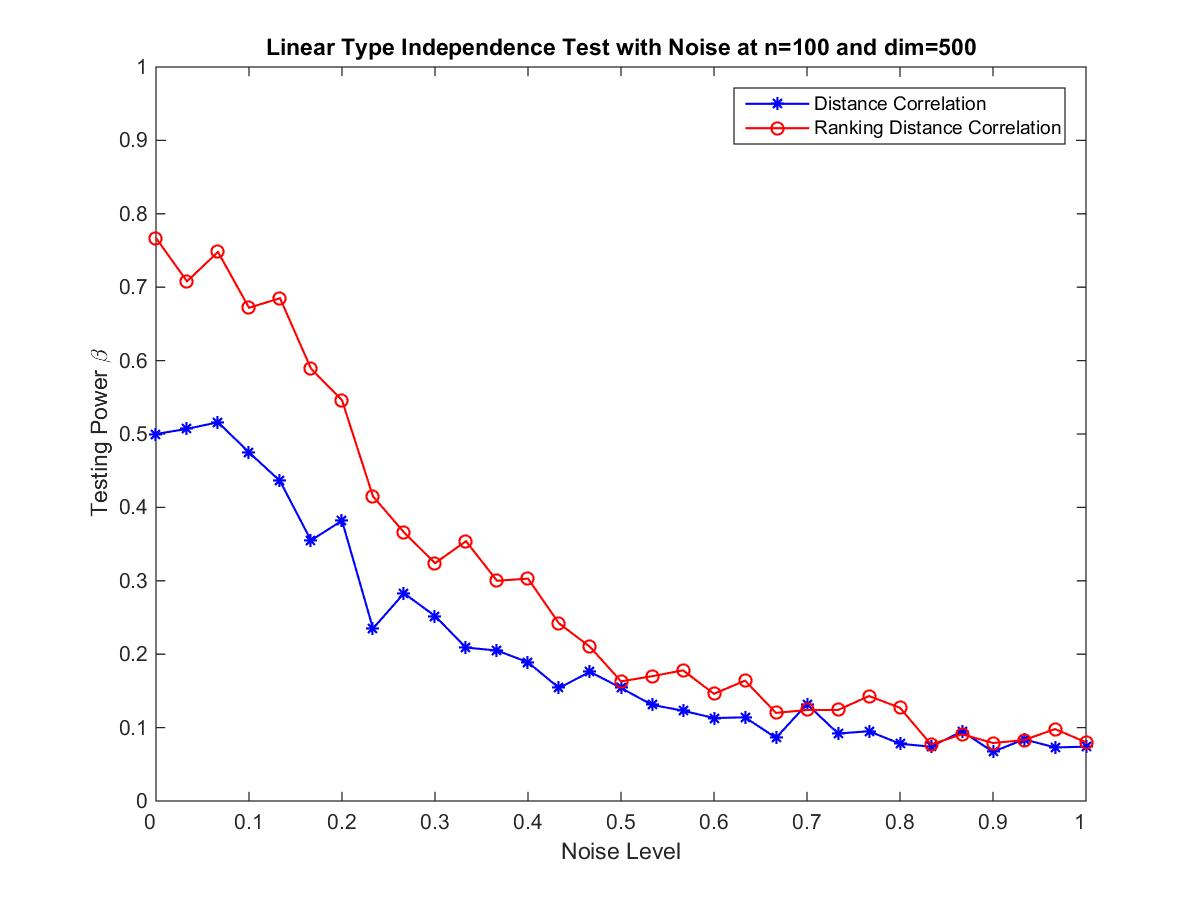
\includegraphics[width=0.5\textwidth]{data/fig2/TibsSimuInd2NoiseType1N100}
}
\hfil
\subfloat[]{
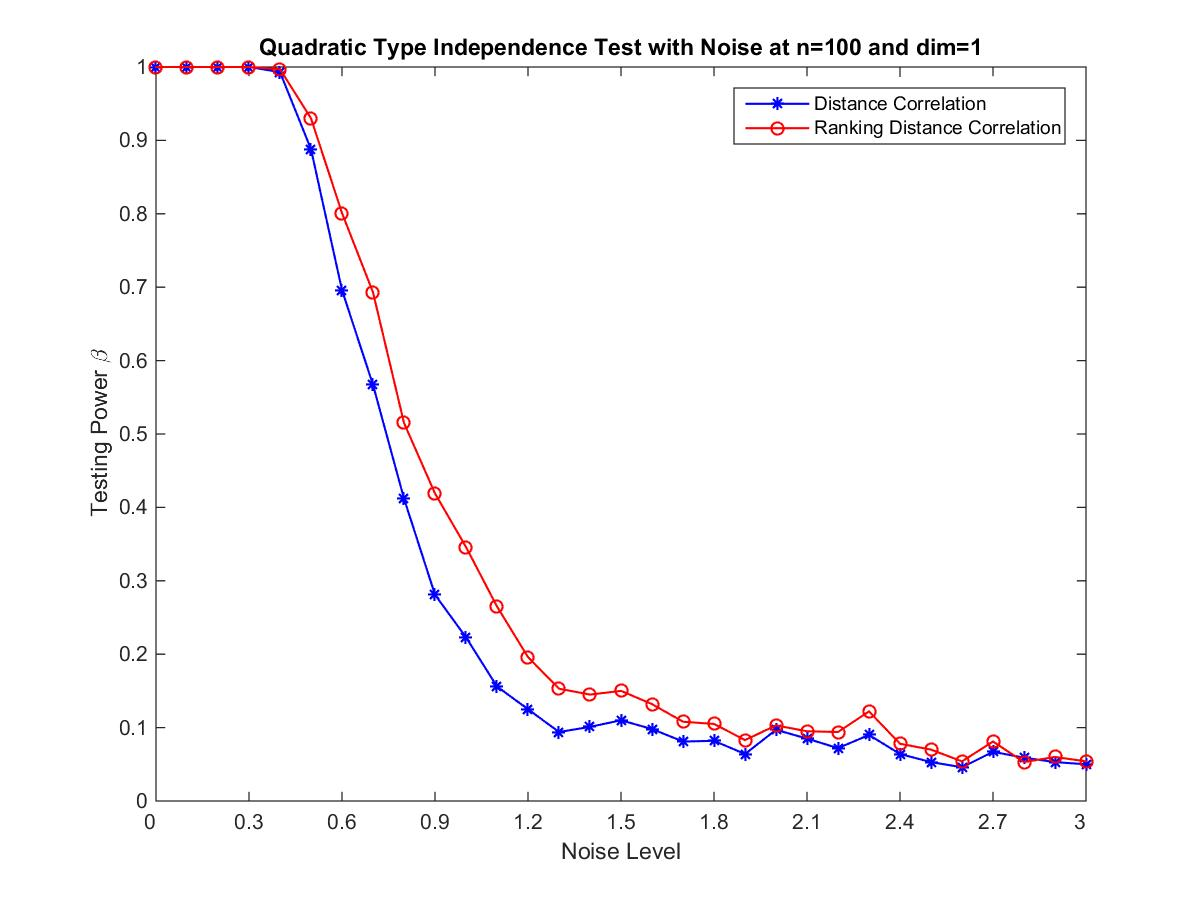
\includegraphics[width=0.5\textwidth]{data/fig2/TibsSimuInd2NoiseType2N100}
}
\hfil
\subfloat[]{
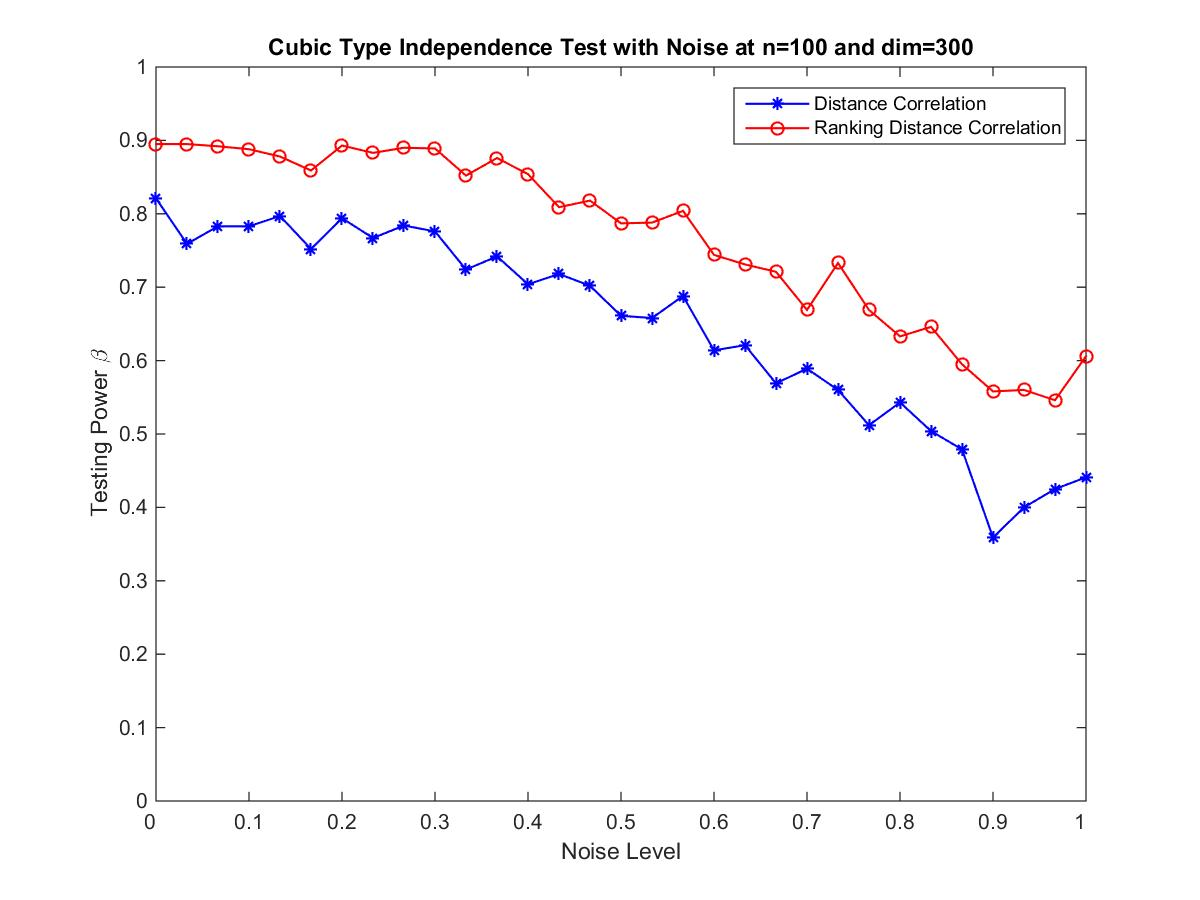
\includegraphics[width=0.5\textwidth]{data/fig2/TibsSimuInd2NoiseType3N100}
}
\hfil
\subfloat[]{
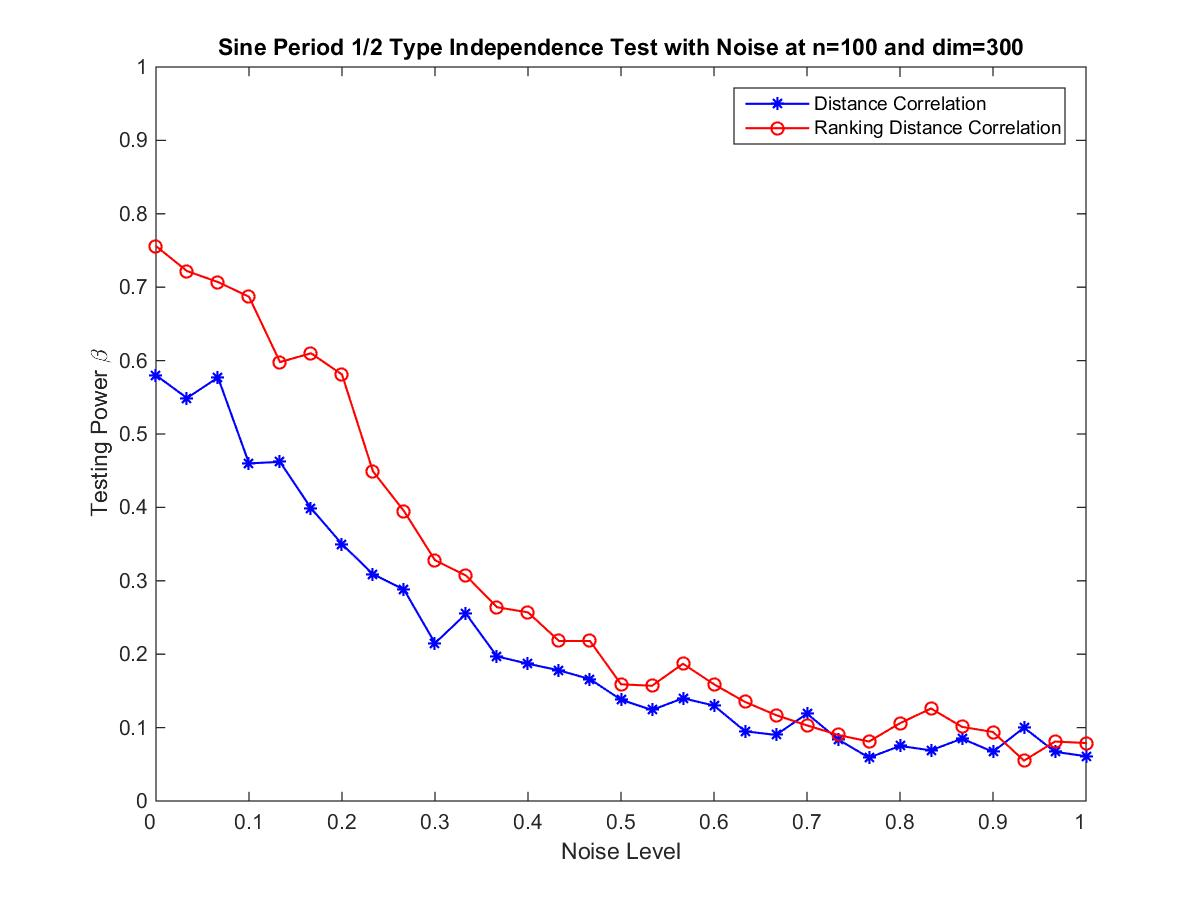
\includegraphics[width=0.5\textwidth]{data/fig2/TibsSimuInd2NoiseType4N100}
}
\hfil
\subfloat[]{
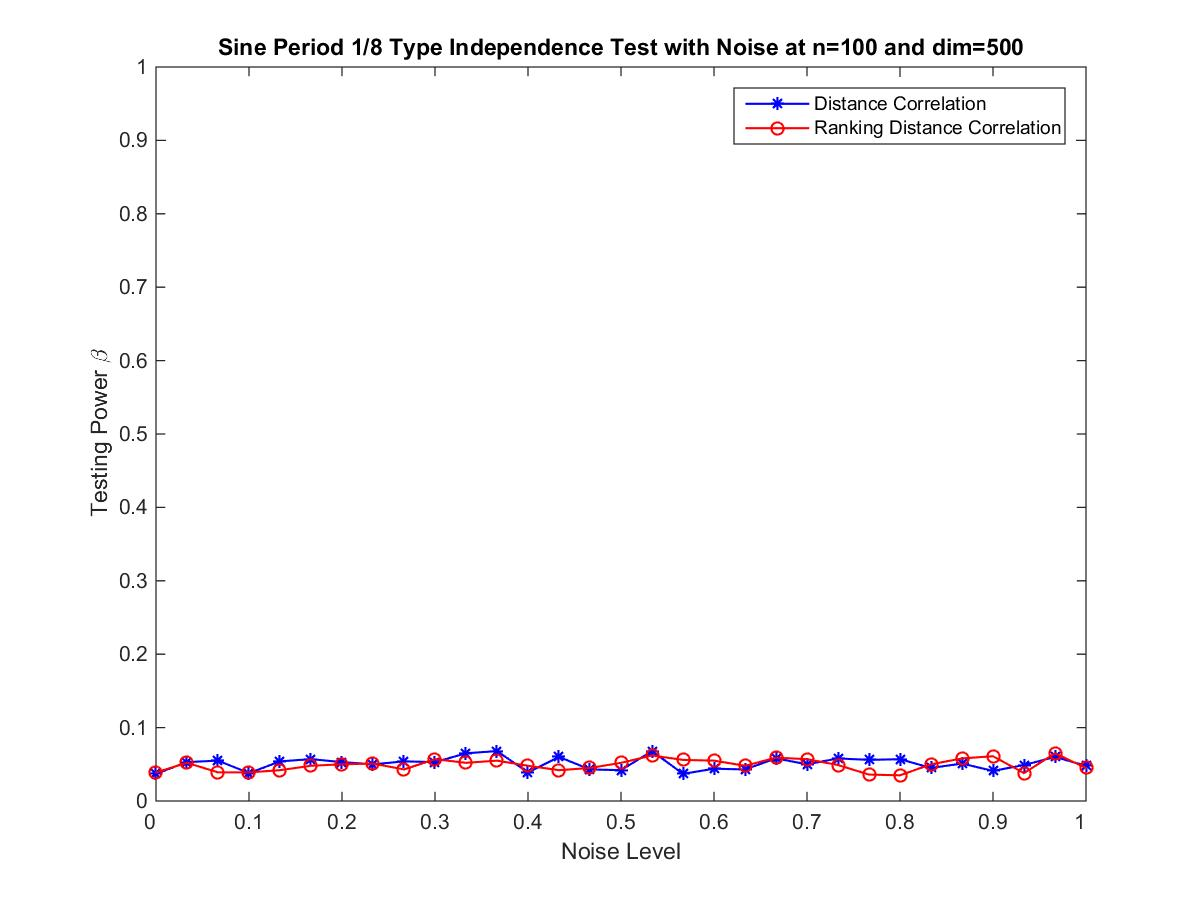
\includegraphics[width=0.5\textwidth]{data/fig2/TibsSimuInd2NoiseType5N100}
}
\hfil
\subfloat[]{
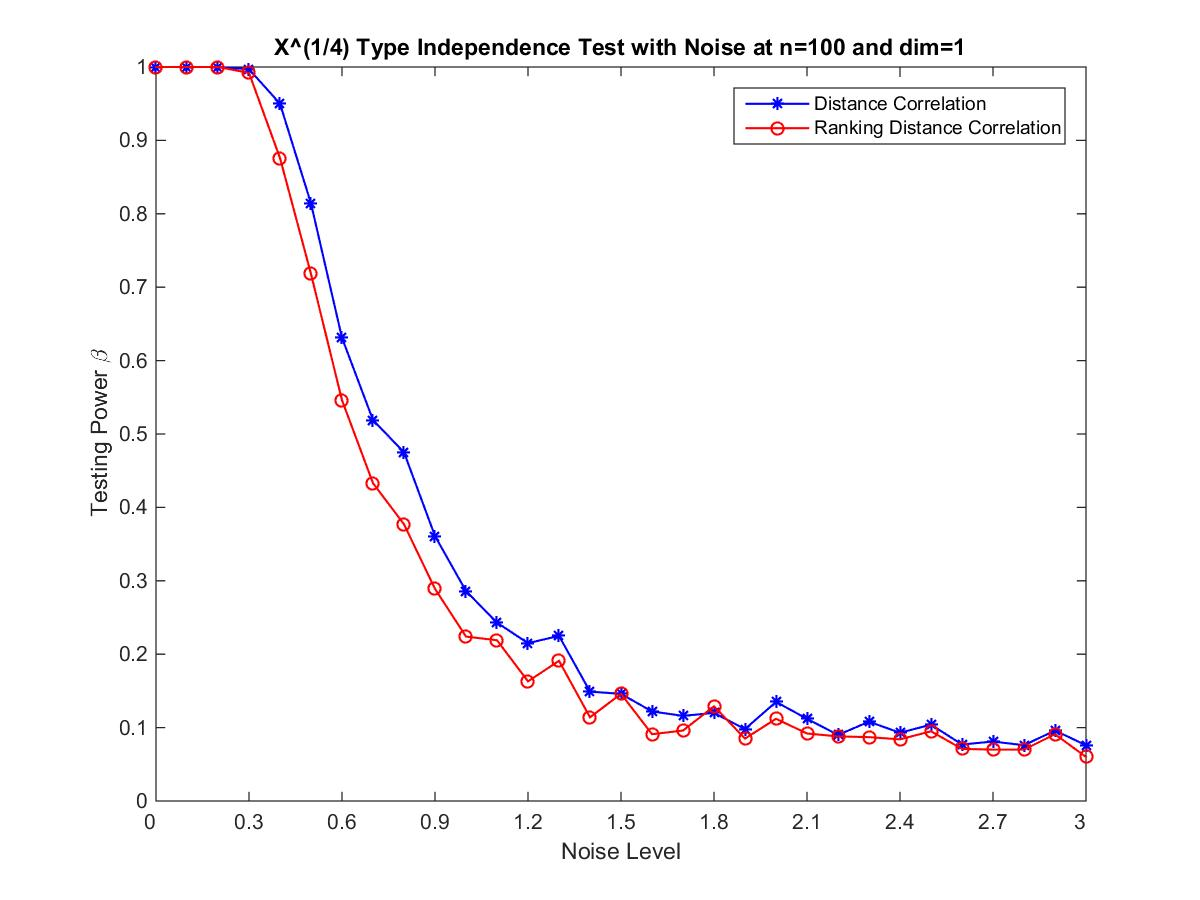
\includegraphics[width=0.5\textwidth]{data/fig2/TibsSimuInd2NoiseType6N100}
}
\caption{Testing Powers w.r.t. Increasing Noise}
\label{}
\end{figure}

\begin{figure}[htbp]
\subfloat[]{
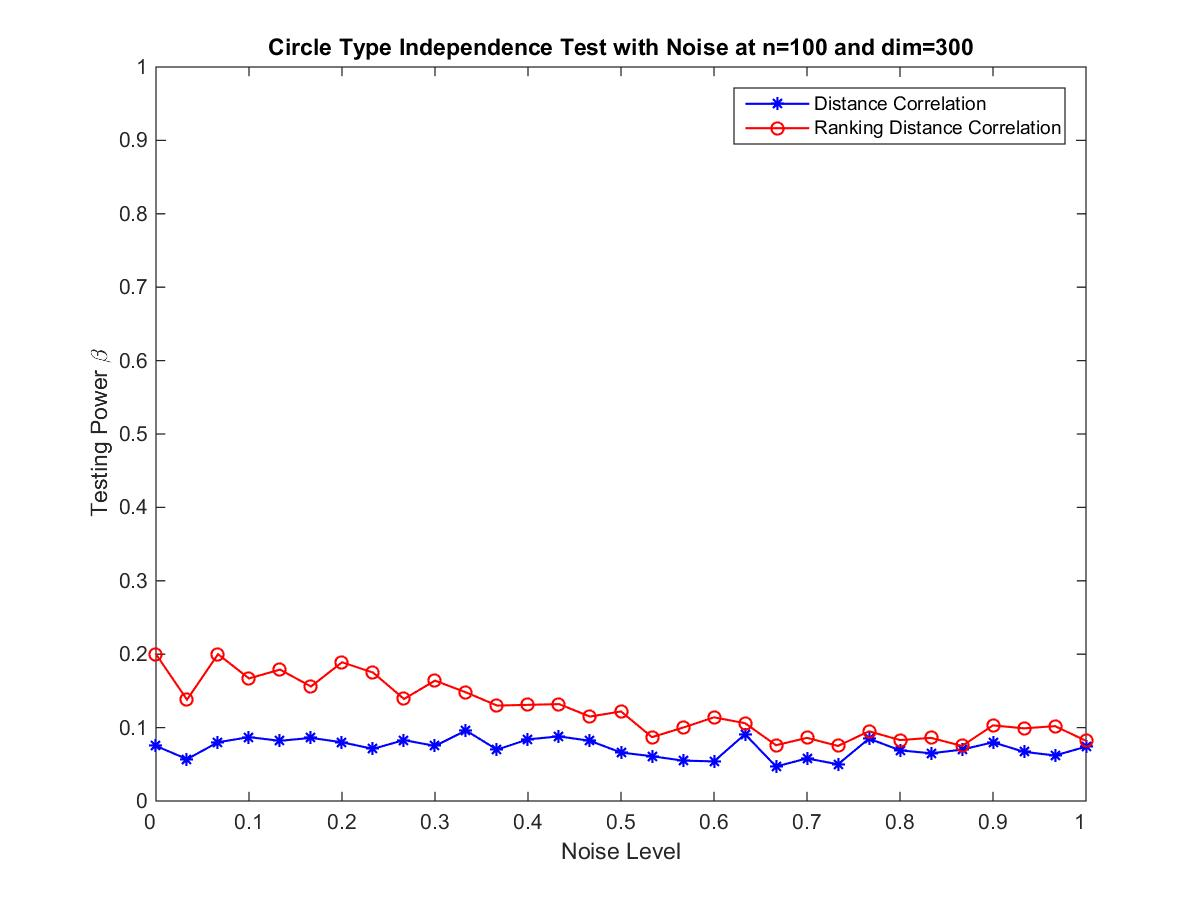
\includegraphics[width=0.5\textwidth]{data/fig2/TibsSimuInd2NoiseType7N100}
}
\hfil
\subfloat[]{
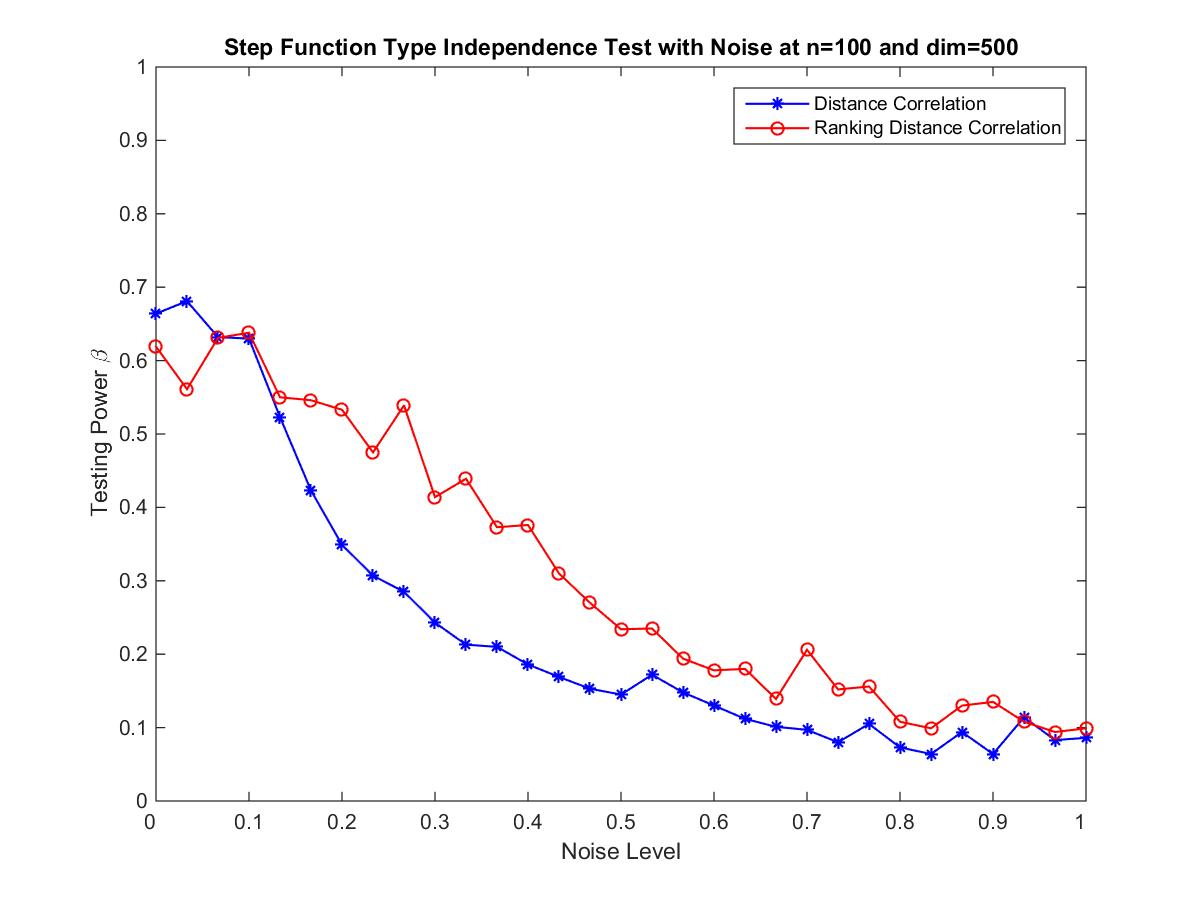
\includegraphics[width=0.5\textwidth]{data/fig2/TibsSimuInd2NoiseType8N100}
}
\hfil
\subfloat[]{
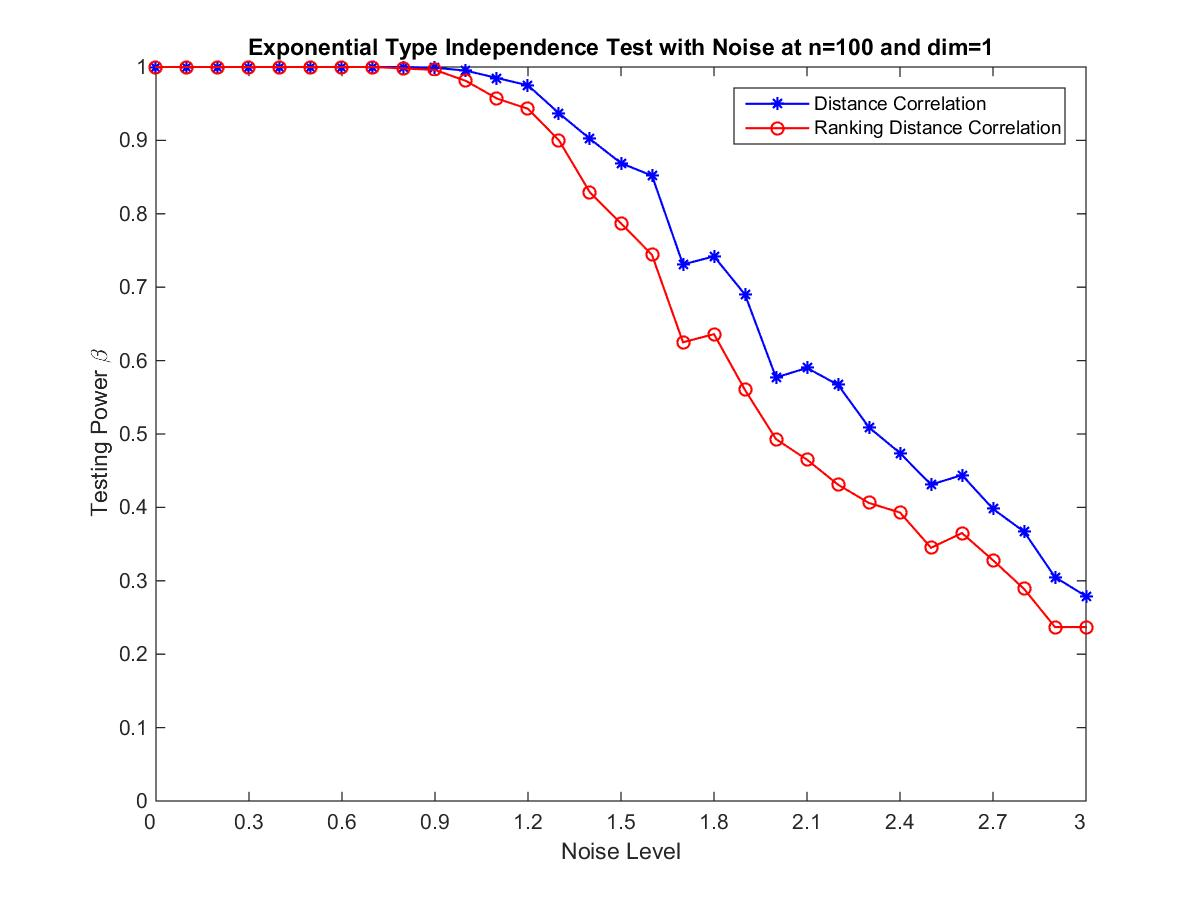
\includegraphics[width=0.5\textwidth]{data/fig2/TibsSimuInd2NoiseType9N100}
}
\hfil
\subfloat[]{
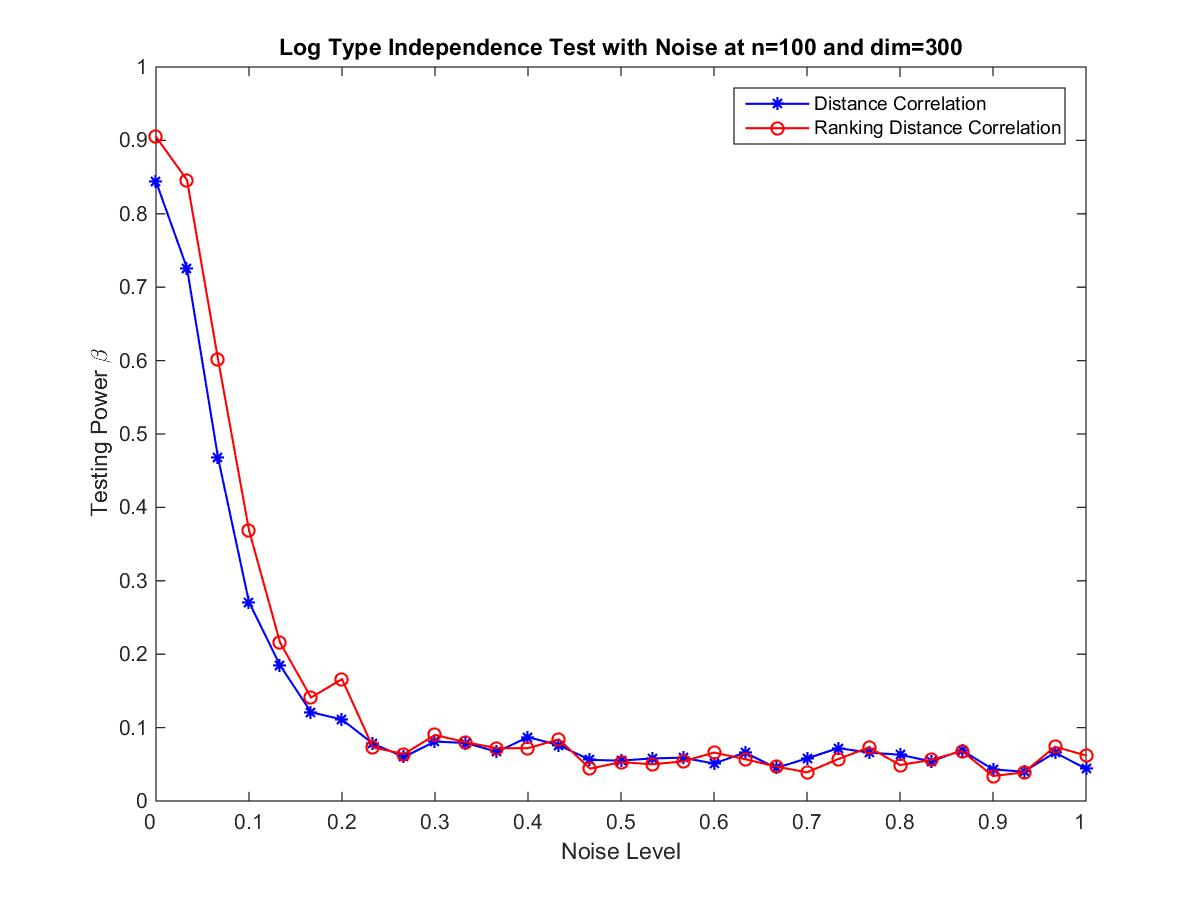
\includegraphics[width=0.5\textwidth]{data/fig2/TibsSimuInd2NoiseType10N100}
}
\caption{Testing Powers w.r.t. Increasing Noise}
\label{}
\end{figure}


%\bibliographystyle{ieeetr}
%\bibliography{references}

\end{document}